\chapter{Пример работы программы}

На рисунке~\ref{fig:int} показан пример работы программы. 
\begin{figure}[h]
	\centering
	
\includegraphics[width=0.8\textwidth]{images/examples/interface.png}
	\caption{Ввод данных в интерфейс приложения}
	\label{fig:int}
\end{figure}

Программа по конвейерному принципу обрабатывает $URL$ адреса рецептов и записывает логи в папку $logs$. У каждого этапа свой лог-файл:
\begin{itemize}
    \item[---] общий лог-файл -- $common.log$;
    \item[---] чтение $HTML$ контента с $URL$ -- $reader.log$;
    \item[---] парсинг $HTML$ контента -- $parser.log$;
    \item[---] запись рецепта в БД -- $writer.log$ 
\end{itemize}

На рисунках~\ref{fig:com}~--~\ref{fig:wri} представлены примеры лог-файлов.

\begin{figure}[h]
	\centering
	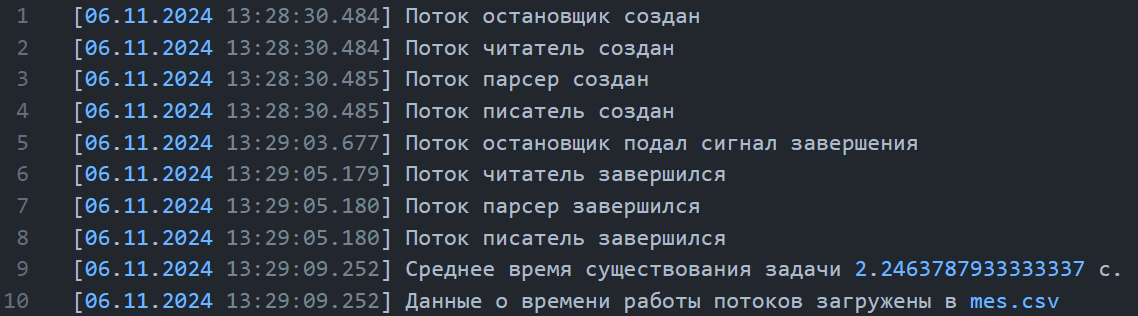
\includegraphics[width=0.8\textwidth]{images/examples/common_log.png}
	\caption{Лог-файл $common.log$}
	\label{fig:com}
\end{figure}

\begin{figure}[h]
	\centering
	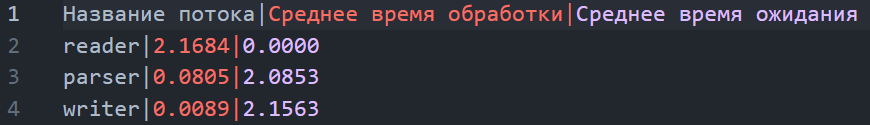
\includegraphics[width=0.8\textwidth]{images/examples/mes_table.png}
	\caption{Данные из файла $mes.csv$}
	\label{fig:com}
\end{figure}

\begin{figure}[h]
	\centering
	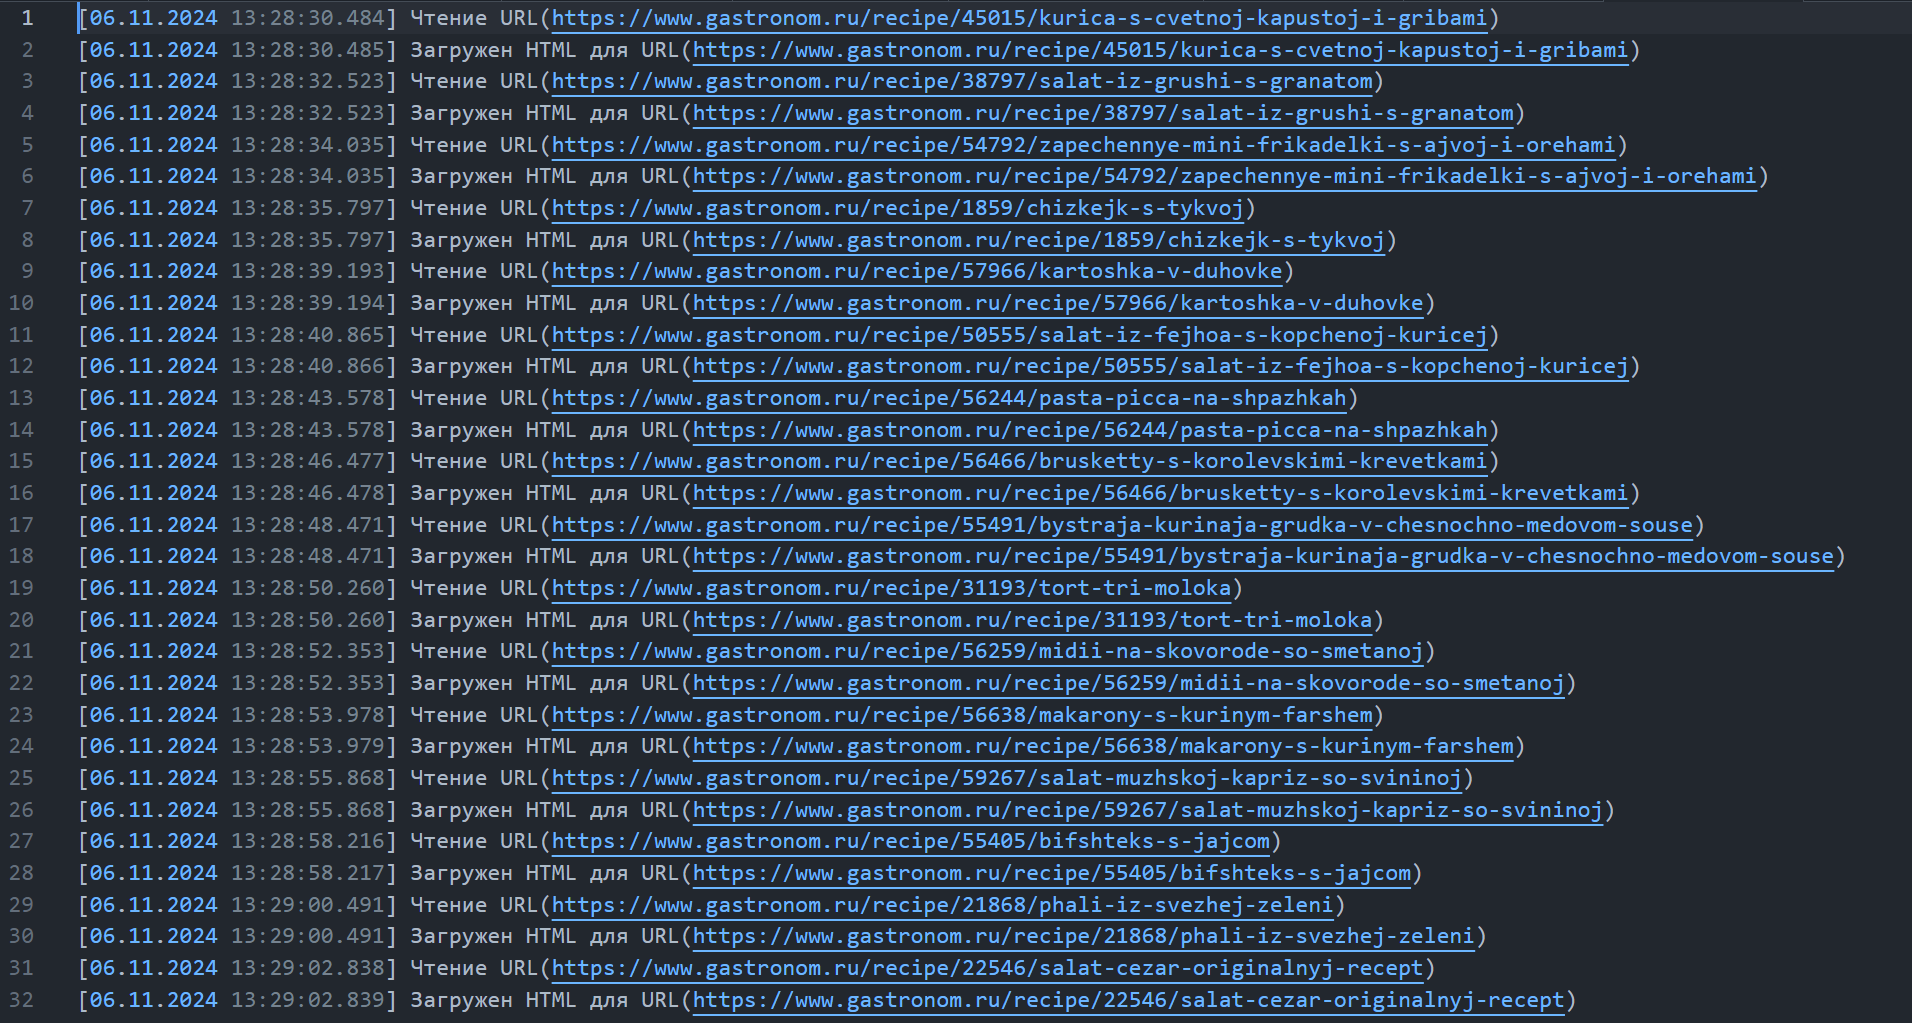
\includegraphics[width=0.8\textwidth]{images/examples/reader_log.png}
	\caption{Лог-файл $reader.log$}
	\label{fig:read}
\end{figure}

\begin{figure}[h]
	\centering
	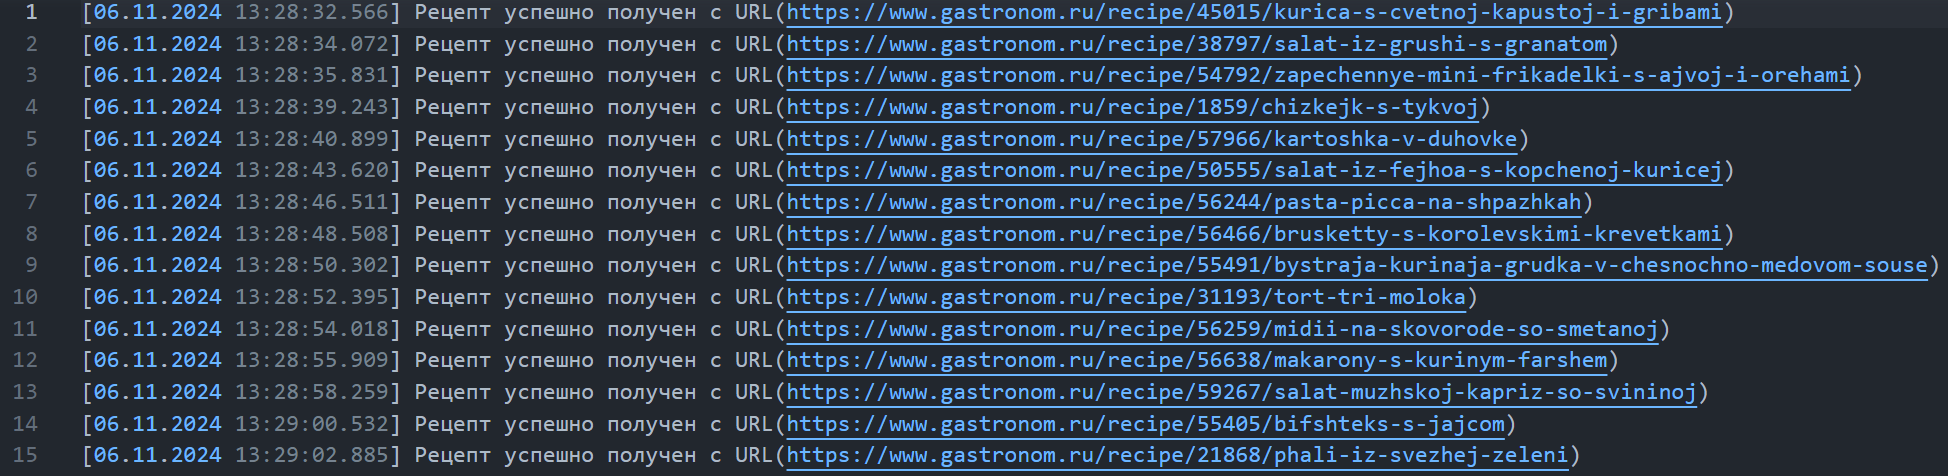
\includegraphics[width=0.8\textwidth]{images/examples/parser_log.png}
	\caption{Лог-файл $parser.log$}
	\label{fig:par}
\end{figure}

\begin{figure}[h]
	\centering
	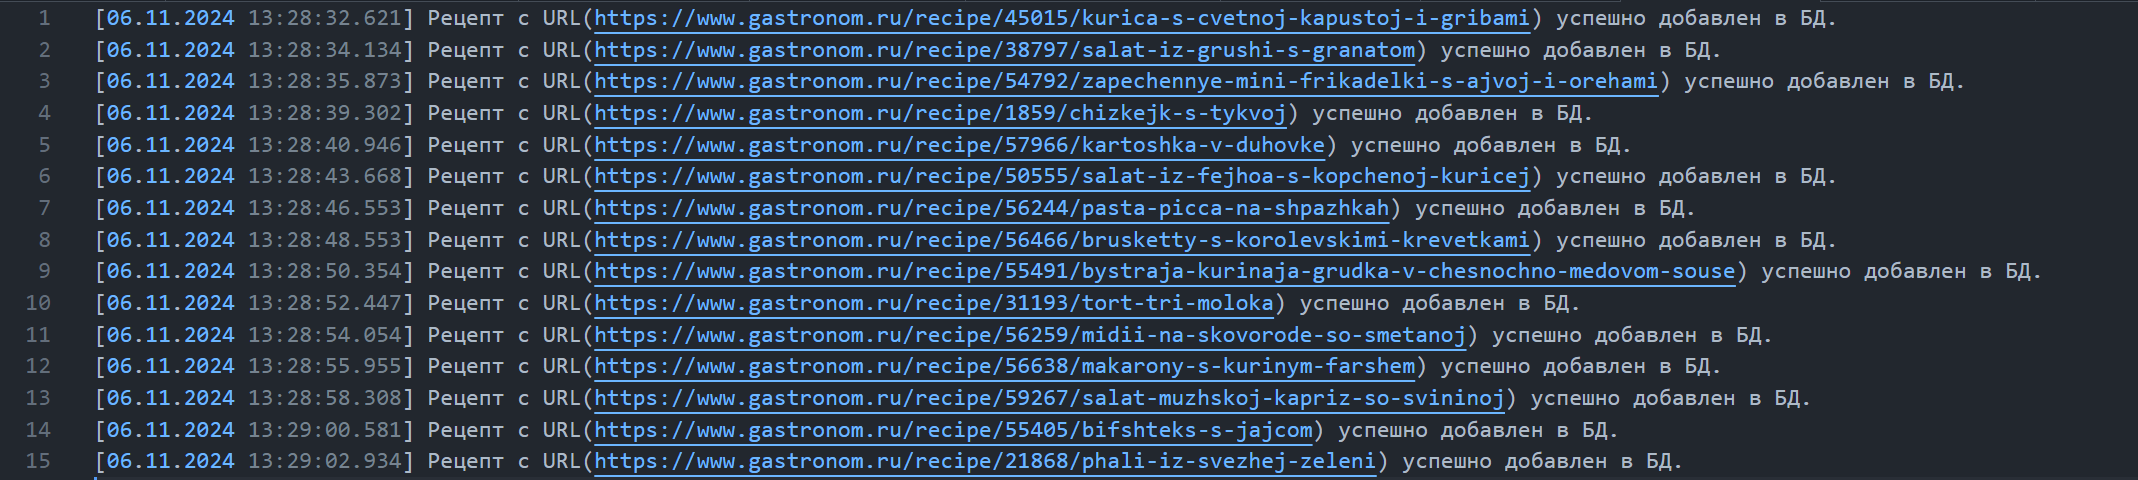
\includegraphics[width=0.8\textwidth]{images/examples/writer_log.png}
	\caption{Лог-файл $writer.log$}
	\label{fig:wri}
\end{figure}

\clearpage

Пример полученной БД, записанной в файле $recipes.db$ представлен на рисунке~\ref{fig:db}

\begin{figure}[h]
	\centering
	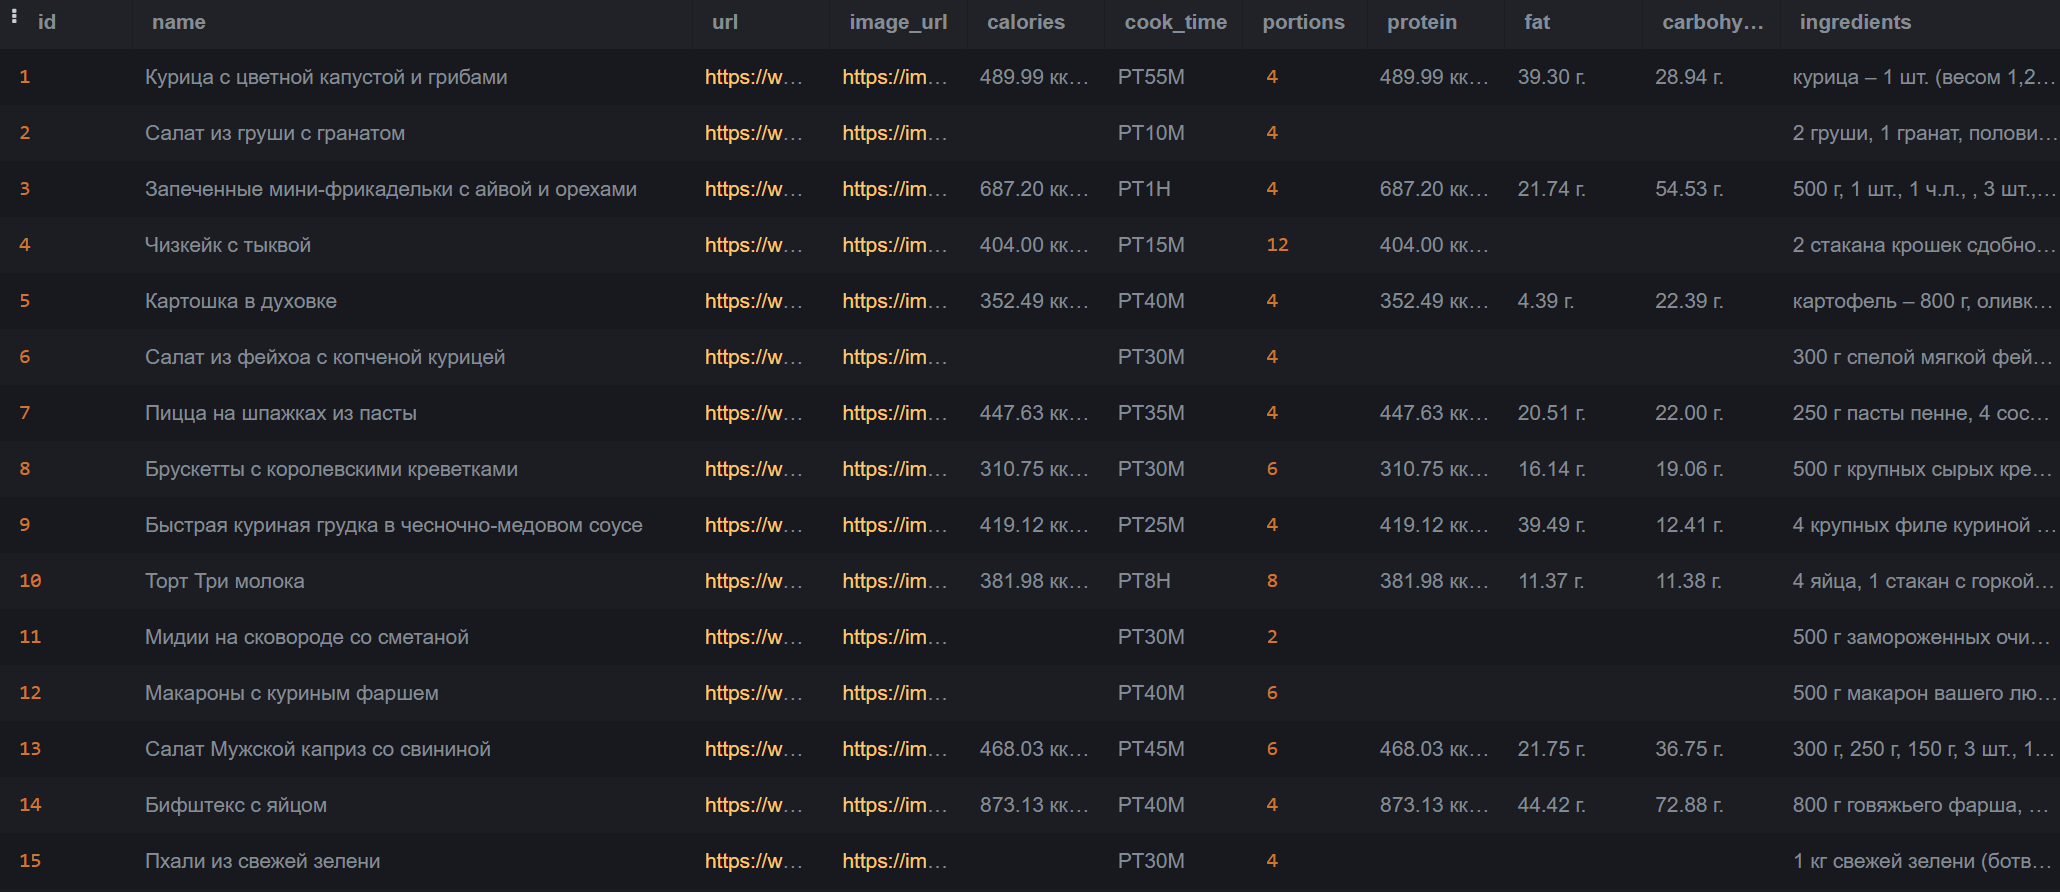
\includegraphics[width=0.8\textwidth]{images/examples/db_example.png}
	\caption{БД из файла $recipes.db$}
	\label{fig:db}
\end{figure}